% covtl-sandhi-guide.tex — didactic guide to covtl-sandhi v0.1.0
% US English, pdflatex, report class. Compile: pdflatex x2.
%
% Sources (nothing invented): covtl-sandhi v0.1.0 README.md / README.fr.md,
% INSTALL.txt, CHANGELOG.md, sandhi/base.py, sandhi/__init__.py, the six
% language modules sandhi/{fr,en,it,es,pt,de}.py (docstrings + tables),
% tests/test_sandhi.py, and README_LIAISON.md of the 5-language v3 pack.

\documentclass[11pt,a4paper]{report}

\usepackage[utf8]{inputenc}
\usepackage[T1]{fontenc}
\usepackage{lmodern}
\usepackage[british]{babel}
\usepackage[margin=2.5cm]{geometry}
\usepackage{booktabs}
\usepackage{longtable}
\usepackage{array}
\usepackage{xcolor}
\usepackage{graphicx}
\usepackage{enumitem}
\usepackage{tikz}
\usetikzlibrary{arrows.meta,positioning,shapes.geometric}
\usepackage[colorlinks=true,linkcolor=blue!45!black,urlcolor=blue!55!black,
            citecolor=blue!45!black]{hyperref}

\setlength{\emergencystretch}{3em}

\newcommand{\smp}[1]{\texttt{#1}}          % inline SAMPA / code
\newcommand{\tld}{\textasciitilde{}}      % the SAMPA nasal tilde
\newcommand{\pkg}{\texttt{covtl-sandhi}}
\newcommand{\pipe}{\texttt{covtl-pipeline}}

\hypersetup{pdftitle={covtl-sandhi v0.1.0 — A Didactic Guide},
            pdfauthor={covtl-sandhi contributors},
            pdfsubject={Inter-word sandhi for the COVTL pipeline languages}}

\title{\textbf{covtl-sandhi v0.1.0}\\[2mm]
       \large A Didactic Guide to Inter-Word Sandhi\\
       in the COVTL Pipeline Languages (fr, en, it, es, pt, de)}
\author{covtl-sandhi contributors}
\date{November 2026 \quad$\cdot$\quad GPL-3.0-or-later}

\begin{document}
\maketitle

\begin{abstract}
\noindent
This guide documents \pkg{} v0.1.0, the standalone package of
\emph{inter-word sandhi} rules for the six languages of the
\pipe{} articulatory speech-synthesis pipeline. It is written for a
pipeline user who knows phonetics but not this code base. We explain
what inter-word sandhi is and why a strictly word-by-word grapheme-to-phoneme
(g2p) conversion can never produce it, how the package is wired into the
pipeline through the two-branch architecture (hook + rules package), how the
three historical modes (\smp{g2p}, \smp{post}, \smp{pre}) differ in fidelity,
and — chapter by chapter — every rule that each of the six language modules
actually applies, with step-by-step derivations from orthography to engine
SAMPA. Coverage levels, editable data tables, known limits, installation and
verification complete the picture. Every rule and every example cited here is
taken from the package sources (README, CHANGELOG, module docstrings, tests)
and from the \smp{README\_LIAISON.md} of the historical five-language patch;
nothing is invented. SAMPA transcriptions are set in monospace.
\end{abstract}

\tableofcontents

% ===========================================================================
\chapter{Introduction: What Is Inter-Word Sandhi?}
% ===========================================================================

\section{The phenomenon}

\emph{Sandhi} is the family of phonological modifications that happen at
boundaries between linguistic units. \emph{Inter-word sandhi} (French
\emph{liaison}, cross-word sandhi) is the part of it that happens
\emph{at word boundaries inside a phrase}. Six examples, one per language of
the package:

\begin{center}\small
\begin{tabular}{@{}llll@{}}
\toprule
language & phenomenon & example & isolated $\rightarrow$ connected \\
\midrule
fr & latent consonant (liaison) & ``faut il'' & \smp{fo.i} $\rightarrow$ \smp{fo.til} \\
en & a$\rightarrow$an + onset linking / linking-r & ``far away'' & \smp{faR.@.we} $\rightarrow$ \smp{fa.R@.we} \\
it & raddoppiamento sintattico + euphonic \emph{d} & ``a casa'' & \smp{a.ka.sa} $\rightarrow$ \smp{a.kka.sa} \\
es & enlace + y$\rightarrow$e / o$\rightarrow$u & ``los amigos'' & \smp{los.a.mi.gos} $\rightarrow$ \smp{lo.sa.mi.gos} \\
pt & encadeamento + EP voicing & ``os amigos'' & \smp{oS.@.mi.guS} $\rightarrow$ \smp{o.Z@.mi.guS} \\
de & Glottalversatz (anti-liaison) & ``ein Apfel'' & \smp{ajn.a.pf@l} $\rightarrow$ \smp{ajn a.pf@l} \\
\bottomrule
\end{tabular}
\end{center}

In every case the modification is triggered by \emph{the pair} (the left word
\textbf{W1} followed by the right word \textbf{W2}): a consonant that is
written but mute at the end of W1 surfaces as the onset of W2 (French), an
article takes \emph{n} before a vowel (English), an initial consonant
geminates after a trigger word (Italian), a final consonant migrates into the
onset of the next syllable (Spanish, Portuguese), or — the deliberate mirror
image — a glottal boundary \emph{separates} the two words instead of linking
them (German).

\section{Why a word-by-word g2p cannot produce it}

The pipeline — like every text-to-SAMPA front end built as a per-word
transducer — converts \emph{one word at a time}. This is by design: a clean
per-word g2p (lexicon $\rightarrow$ exceptions $\rightarrow$ rules) is
testable, cacheable and maintainable. But the information needed for
inter-word sandhi simply \emph{does not exist inside a single word}:

\begin{itemize}[nosep]
  \item the latent consonant of French \emph{faut} is mute in isolation
        (\smp{fo}); nothing in the isolated word tells you that a \smp{t}
        must appear when \emph{il} follows;
  \item the Spanish final \smp{s} of \smp{los} is a coda in isolation; only
        the vowel-initial \smp{a.mi.gos} on its right turns it into an onset;
  \item the Italian trigger status of \emph{citt\`a} (written final accent)
        is a property of W1, but the gemination lands on W2.
\end{itemize}

The guide's opening example says it all: a perfect per-word g2p gives
\smp{fo.i} for ``faut il''; the correct connected form is \smp{fo.til}.
Whatever is missing lies \emph{between} the two per-word tokens — exactly
where a word-by-word transducer never looks. This is why the pipeline needs a
separate, pair-aware layer: the \pkg{} package documented here.

\section{Where covtl-sandhi sits in covtl-pipeline}

\pkg{} lives strictly in the \textbf{text/g2p layer} of the pipeline, next to
the expressive-prosody patch. It rewrites text or SAMPA \emph{before} the
synthesis engine is called. Three architectural invariants hold everywhere
(module docstrings, README, CHANGELOG):

\begin{enumerate}
  \item \textbf{The synthesis engine is never modified.} The engine modules
        (\smp{syltraj}, \smp{polar}, \smp{gesture}, \smp{build\_phrase\_tract},
        \dots) receive an ordinary SAMPA string. It was verified on a pipeline
        clone that linked forms such as \smp{mO\tld.na.mi} pass
        \smp{syltraj} without the \smp{V\tld.V} nasal collapse: the linking
        consonant interposes itself between the two vowels.
  \item \textbf{Every language is respected.} Each rule table applies only to
        word pairs of its own language; any other profile is a no-op with a
        warning. The English profile is covered by its own module (new in
        v0.1.0), not ignored.
  \item \textbf{Compatibility with the expressive-prosody patch.} The sandhi
        key (inserted or displaced) is always a \emph{consonant}, never a
        syllabic nucleus, and nothing is ever inserted across a pause
        (\smp{\%}, \smp{|}, comma). Section~\ref{sec:invariant} explains why
        this matters for the F0 plans.
\end{enumerate}

\section{Notation and how to read this guide}

Engine SAMPA is set in monospace: \smp{fo.til}. Within a phrase string the
engine uses the following separators (mirrored from the pipeline g2p
conventions, cf.\ the module docstrings):

\begin{center}
\begin{tabular}{@{}ll@{}}
\toprule
symbol & meaning \\
\midrule
\smp{.} & syllable link (inside a word, and between linked words of a phrase) \\
\smp{(space)} & word boundary — a short pause / re-articulation \\
\smp{|} (with spaces) & sentence boundary \\
\smp{\%} & breath pause inserted by the expressive-prosody plan \\
\bottomrule
\end{tabular}
\end{center}

Chapters~\ref{chap:arch}–\ref{chap:method} cover architecture and method;
Chapters~\ref{chap:fr}–\ref{chap:de} are one chapter per language, each
opening with a spoken example and then listing \emph{all} trigger classes,
exceptions and derivations the module implements;
Chapters~\ref{chap:levels}–\ref{chap:install} cover coverage levels, editable
tables, limits, and installation. Sources are cited inline as file names; the
phonological references of each module are collected in the bibliography.

% ===========================================================================
\chapter{Architecture: Branch A (Hook) + Branch B (This Package)}
\label{chap:arch}
% ===========================================================================

\section{Overview}

The distribution splits cleanly into two branches that can be installed
independently:

\begin{itemize}
  \item \textbf{Branch A — the hook}: a light git patch
        \smp{patch/covtl-pipeline-sandhi-hook.patch} applied to the
        \emph{pipeline} repository. It adds a stub package
        \smp{vtl\_synth/utils/sandhi/} (with \smp{SANDHI\_FULL = False}:
        every entry point is the identity) and the command-line options
        \smp{-{}-sandhi} and \smp{-{}-sandhi-mode}.
  \item \textbf{Branch B — the rules}: the \pkg{} package itself
        (this distribution): six language modules
        (\smp{fr.py}, \smp{en.py}, \smp{it.py}, \smp{es.py}, \smp{pt.py},
        \smp{de.py}), the shared \smp{base.py}, the editable views
        \smp{data/*.txt}, and the standalone test suite.
\end{itemize}

\begin{figure}[htbp]
\centering
\resizebox{\textwidth}{!}{%
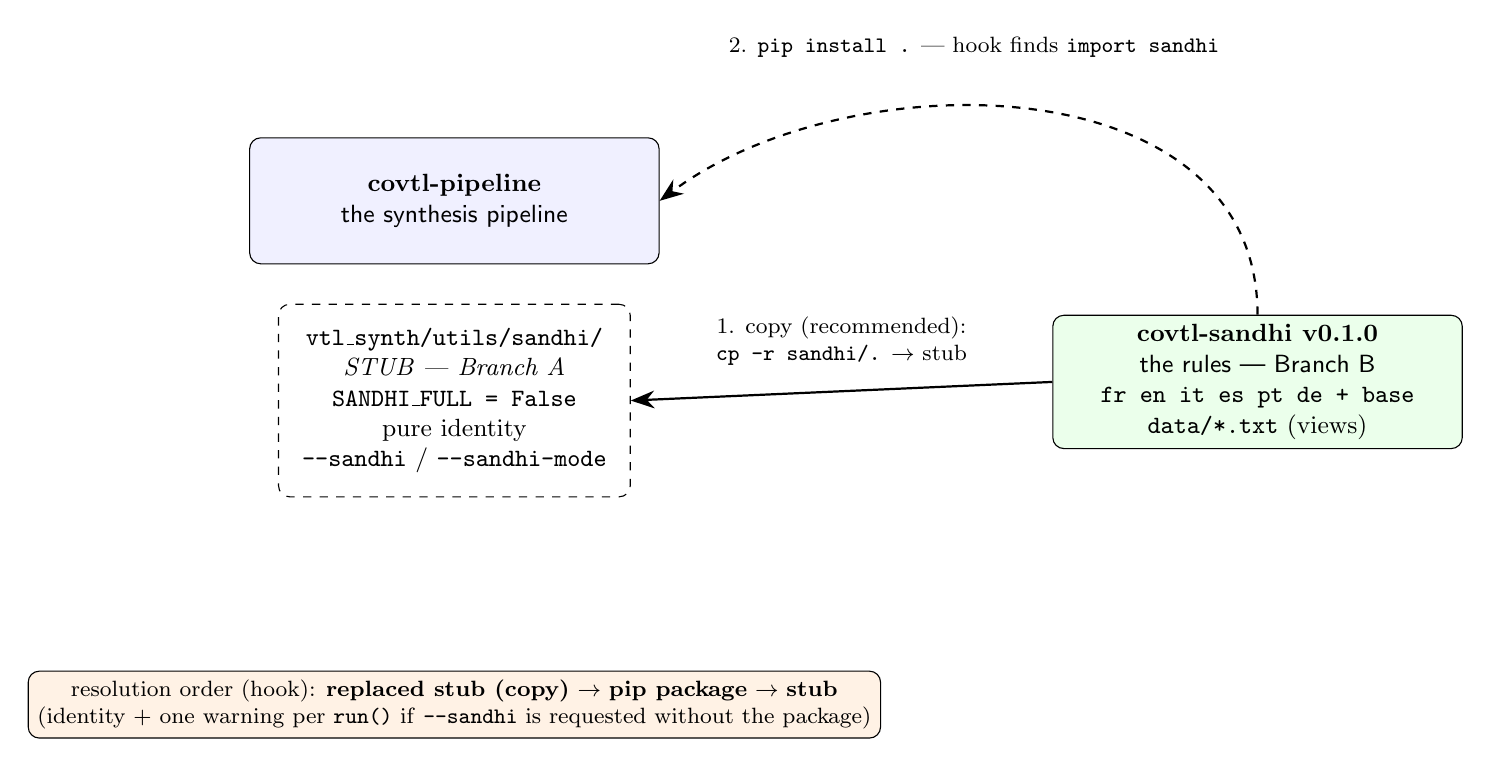
\begin{tikzpicture}[
  font=\small,
  box/.style={draw, rounded corners, fill=blue!6, align=center,
              minimum width=52mm, minimum height=16mm},
  inner/.style={draw, dashed, rounded corners, fill=white, align=center,
                inner sep=3mm},
  arrow/.style={-{Stealth[length=3mm]}, thick},
  dasharrow/.style={-{Stealth[length=3mm]}, thick, dashed}]
  \node[box] (pipe) at (0,0)
    {\textbf{covtl-pipeline}\\\textsf{the synthesis pipeline}};
  \node[inner, below=5mm of pipe.south, anchor=north] (stub)
    {\texttt{vtl\_synth/utils/sandhi/}\\\emph{STUB — Branch A}\\
     \texttt{SANDHI\_FULL = False}\\ pure identity\\
     \texttt{-{}-sandhi} / \texttt{-{}-sandhi-mode}};
  \node[box, fill=green!8] (pkg) at (10.2,-2.3)
    {\textbf{covtl-sandhi v0.1.0}\\\textsf{the rules — Branch B}\\
     \texttt{fr en it es pt de + base}\\\texttt{data/*.txt} (views)};
  % 1) copy: straight arrow pkg -> stub, label above, in the free gap
  \draw[arrow] (pkg.west) -- (stub.east)
    node[midway, above=2mm, align=center, font=\footnotesize]
      {1. copy (recommended):\\ \texttt{cp -r sandhi/.} $\to$ stub};
  % 2) pip: arc over the free top area (explicit control points)
  \draw[dasharrow] (pkg.north) .. controls +(0,3.2) and +(2.4,1.8) ..
    (pipe.east);
  \node[font=\footnotesize, anchor=south] at (6.6,1.7)
    {2. \texttt{pip install .} — hook finds \texttt{import sandhi}};
  \node[draw, rounded corners, fill=orange!10, align=center, font=\footnotesize,
        below=22mm of stub.south, anchor=north] (res)
    {resolution order (hook): \textbf{replaced stub (copy)} $\rightarrow$
     \textbf{pip package} $\rightarrow$ \textbf{stub}\\
     (identity + one warning per \texttt{run()} if \texttt{-{}-sandhi}
     is requested without the package)};
\end{tikzpicture}%
}
\caption{Branch A / Branch B architecture and the hook's resolution chain.}
\label{fig:arch}
\end{figure}

\section{Branch A: the hook, and the bit-identical guarantee}

The hook patch is deliberately boring: the stub it installs contains the same
function signatures as the full package, but every function is the identity
(\smp{SANDHI\_FULL = False}), and the new CLI options default to
\smp{-{}-sandhi off}. The consequence, verified on a clean clone of the
pipeline (\smp{main} @ \smp{41f6571}, \emph{INSTALL.txt}):

\begin{itemize}
  \item the patch applies cleanly; the repository test suite goes from
        \textbf{155 passed} (virgin clone) to \textbf{165 passed} with the
        hook — exactly the $+10$ hook tests, \textbf{0 regressions}, the
        3 pre-existing failures unchanged;
  \item with the hook alone the pipeline outputs are
        \textbf{bit-identical} to the unpatched repository: the hook is
        invisible by default.
\end{itemize}

This is what makes the hook safe to merge and ship independently of the
rules: nothing changes until Branch B is installed \emph{and} the user asks
for \smp{-{}-sandhi}.

\section{Branch B: activating the rules}

Two equivalent activations (pick one):

\begin{enumerate}
  \item \textbf{Direct copy (recommended to stay self-contained).} The stub
        folder \emph{already exists} after the hook, so you copy the
        \textbf{content} of the package's \smp{sandhi/} directory — note the
        trailing \smp{/.} in
\begin{verbatim}
cp -r sandhi/.  <pipeline>/vtl_synth/utils/sandhi/
\end{verbatim}
        Without the \smp{/.}, \smp{cp -r sandhi/ dst/} would nest the folder
        one level too deep (\smp{dst/sandhi/...}) and the hook would keep
        finding its stub. (PowerShell equivalent:
        \smp{Copy-Item -Path sandhi\textbackslash* -Destination dst -Recurse -Force}.) The
        package overwrites the stub; the hook now reads
        \smp{SANDHI\_FULL = True}.
  \item \textbf{pip.} \smp{pip install .} installs the package into
        site-packages; if the stub has not been replaced, the hook detects
        the importable \smp{sandhi} package instead.
\end{enumerate}

The full resolution chain is therefore: replaced stub (copy) $\rightarrow$
pip package $\rightarrow$ stub (identity, plus one warning per \smp{run()}
if a sandhi level was requested without any package installed).

% ===========================================================================
\chapter{The Method Inside the Pipeline}
\label{chap:method}
% ===========================================================================

\section{The per-word oracle}

Every module exposes an \emph{oracle}: a function
\smp{oracle(word, g2p) -> token} that returns the SAMPA token of one word.
The oracle is the package's only window onto the pipeline's g2p: the active
g2p is called word by word through its public interface
\smp{(text, warnings) -> str} — there is no import from any \smp{g2p\_*}
module (independence requirement of the framework).

\begin{itemize}
  \item For \textbf{it, es, pt, de, en} the per-word g2p is backed by a
        lexicon (Wikipron for it/es/pt/de, CMUdict for en) and was measured
        exact on the clone: the oracle is the \emph{identity}. It exists for
        architectural symmetry.
  \item For \textbf{fr} the base g2p damages the closed class
        (\emph{il} $\rightarrow$ \smp{i}, \emph{est} $\rightarrow$ \smp{e},
        \emph{petit} $\rightarrow$ \smp{ti}, \emph{plus}
        $\rightarrow$ \smp{py}\dots). The French oracle applies a small
        table of corrections, \smp{\_PRON\_OVERRIDES}
        (\smp{sandhi/fr.py}), \emph{only to words that belong to a liaison
        pair} — the rest of the phrase keeps the base tokens, so
        \smp{off} stays bit-identical:
\begin{center}
\begin{tabular}{@{}llll@{}}
\toprule
word & override & base g2p & comment \\
\midrule
il / ils & \smp{il} & \smp{i} & final \smp{l} recovered \\
elle & \smp{El} & \smp{a} & \\
est & \smp{E} & \smp{e} & open vowel \\
cet & \smp{sE} & \smp{st} & \\
ces & \smp{se} & \smp{se.@.Es} & \\
petit & \smp{p@.ti} & \smp{ti} & \\
plus & \smp{ply} & \smp{py} & \\
second & \smp{s@gO\tld} & \smp{zgO\tld} & \\
huit & adds final \smp{t} & loses it & initial glide kept \\
dernier & \smp{dER.nje} & \smp{dERn.je} & \\
ancien & \smp{a\tld{}sjE} & \smp{a\tld{}sjE\tld} & denasalised \\
certain & \smp{sER.tE} & \smp{sERtE\tld} & denasalised \\
\bottomrule
\end{tabular}
\end{center}
\end{itemize}

\section{Pair planning: from text to pairs}

All modules share the same text-splitting skeleton (a fresh mirror of each
language g2p's conventions; see the regex tables in the modules): sentences
are split on \smp{[.!?;:]+}, comma-parts on \smp{[,--]} (a comma is a
boundary: \emph{a pair never links across it}), words by a per-language
letter class (French keeps the apostrophe — \emph{c'est}; Italian, Spanish,
Portuguese and German do not, mirroring their g2p tokenisers).

\smp{plan\_pairs(text, g2p, level)} then walks every adjacent pair
(\smp{W1}, \smp{W2}) of every comma-part, asks the module's decision
function \emph{``does this pair carry a sandhi, and at which coverage
level?''} and returns the plan: for each pair index, either \smp{None} or a
record (kind, key to insert or displace, both tokens). Pairs may
\emph{chain}: in Italian ``cos\`{\i} come va'' both
cos\`{\i}$\rightarrow$come and come$\rightarrow$va fire; in Spanish
``es un amigo'' the word \emph{un} both receives \smp{s} and loses its
\smp{n}.

\section{SAMPA fusion in slots}

The fusion step (\smp{apply\_liaison\_post} / \smp{apply\_sandhi\_post} in
each module) first \emph{aligns} the plan against a produced SAMPA string:
sequentially, each word's token is found as a slot delimited by \smp{.} or
space (\smp{\_find\_slot}); internal dots of a token (\smp{a.mi.gos}) belong
to the token and never create false slots; the alignment must consume the
sentence exactly (nothing left except \smp{\%} markers). Then, right-to-left
so offsets stay valid, each planned pair is fused:

\begin{itemize}
  \item \textbf{insertion} (fr latent, it geminate/d, en \emph{an}): the key
        is carried by the \emph{right slot}, in onset —
        \smp{['fo','i']} $\rightarrow$ \smp{['fo','ti']};
  \item \textbf{displacement} (es enlace, pt encadeamento, en onset linking):
        the left slot is amputated of its final consonant, which becomes the
        onset of the right slot — \smp{['los','a.mi.gos']}
        $\rightarrow$ \smp{['lo','sa.mi.gos']}; chained groups are
        reconstructed segment by segment;
  \item \textbf{boundary} (de): the right slot receives a \emph{leading
        space} — \smp{['ajn','a.pf@l]} $\rightarrow$
        \smp{['ajn',' a.pf@l']}, and the join
        \smp{join\_words\_keys} does not double the separator.
\end{itemize}

If the gap between the two slots of a pair is anything but \smp{.} or a
space — i.e.\ a \smp{\%} breath pause, a \smp{|} sentence boundary, or a
comma — the pair is skipped. On any alignment failure the whole sentence is
returned unchanged (fail-safe, never a wrong form).

\begin{figure}[htbp]
\centering
\resizebox{0.98\textwidth}{!}{%
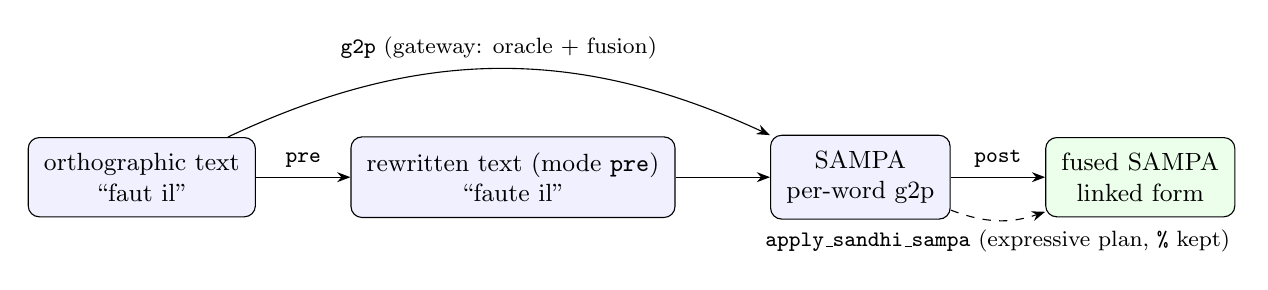
\begin{tikzpicture}[font=\small, node distance=6mm and 12mm,
  stage/.style={draw, rounded corners, fill=blue!6, align=center,
                minimum height=9mm, inner sep=2mm}]
  \node[stage] (text) {orthographic text\\``faut il''};
  \node[stage, right=of text] (preg2p) {rewritten text (mode \smp{pre})\\``faute il''};
  \node[stage, right=of preg2p] (sampa) {SAMPA\\per-word g2p};
  \node[stage, right=of sampa, fill=green!8] (out) {fused SAMPA\\linked form};
  \draw[-{Stealth}] (text) -- node[above, font=\footnotesize] {\smp{pre}} (preg2p);
  \draw[-{Stealth}] (text) to[bend left=25] node[above, font=\footnotesize]
    {\smp{g2p} (gateway: oracle + fusion)} (sampa);
  \draw[-{Stealth}] (preg2p) -- (sampa);
  \draw[-{Stealth}] (sampa) -- node[above, font=\footnotesize] {\smp{post}} (out);
  \draw[-{Stealth}, dashed] (sampa) to[bend right=20]
    node[below, font=\footnotesize] {\smp{apply\_sandhi\_sampa} (expressive plan, \smp{\%} kept)} (out);
\end{tikzpicture}%
}
\caption{The three modes and the expressive path. \smp{g2p} is the
recommended route; \smp{pre} rewrites the text and feeds the plain g2p;
\smp{post} edits an already produced SAMPA.}
\label{fig:modes}
\end{figure}

\section{The three modes and their fidelity trade-offs}

The option \smp{-{}-sandhi-mode} keeps the three historical implementations
of the five-language patch as a user choice (\smp{README\_LIAISON.md},
module docstrings):

\begin{center}
\begin{tabular}{@{}p{14mm}p{47mm}p{22mm}p{47mm}@{}}
\toprule
mode & where it acts & fr ``faut il'' & strengths / limits (measured) \\
\midrule
\smp{pre} & before the g2p: orthographic rewrite of the text
(``faut'' $\rightarrow$ ``faute''); g2p untouched &
\smp{fot.i} &
maximally decoupled; latent lands in \emph{coda} (not onset), small vowel
symbol shifts (\smp{o\tld}/\smp{O\tld}), partial coverage (no correct
respelling for \emph{est}, \emph{petit}, \emph{plus}, \emph{vieux}, \emph{ces},
\emph{plein}, \emph{jamais}, \emph{beaucoup}); no-op for de/en (no spelling
exists). \\[2mm]
\smp{g2p} \textbf{(default, recommended)} & in the g2p layer:
sandhi-aware gateway — per-word oracle + pair fusion with corrected tokens &
\smp{fo.til} &
latent in \emph{onset}, closed-class corrections, chains with
\smp{-{}-expressive}; the only insertion point that sees both the pair and
the pronunciation. \\[2mm]
\smp{post} & after the g2p: pure SAMPA post-processor (insertion only,
base g2p totally untouched) &
\smp{fo.ti} &
most decoupled after the fact; inherits the base g2p per-word defects (here
\emph{il} $\rightarrow$ \smp{i}: the \smp{l} is missing — inserting cannot
repair a token). \\
\bottomrule
\end{tabular}
\end{center}

The method search that concluded with this design is quoted in
\smp{README\_LIAISON.md}: the word boundary is visible \emph{neither}
upstream — spelling does not reliably encode the phenomenon (and German
encodes nothing at all) — \emph{nor} downstream — the produced SAMPA has
lost the boundary, and the g2p's per-word defects cannot be repaired by
insertion. The g2p layer is the only place where both are available. For
it/es/pt/de/en the oracle is the identity, so \smp{g2p} and \smp{post}
produce identical outputs there; the difference is architectural. In
\smp{pre} mode the gateway returns the g2p output \emph{over the rewritten
text}; \smp{sandhi\_rewrite\_text} returns the rewritten orthography alone,
so the expressive planner can be fed the same respelled text as the monotone
path.

\section{The expressive path and the key invariant}
\label{sec:invariant}

The expressive-prosody patch plans F0 over the phrase \emph{before} the
final synthesis, and its plan indexes syllable \emph{nuclei}. The expressive
entry point of the package is therefore
\begin{center}
\smp{apply\_sandhi\_sampa(lang, text, sampa, g2p, level, mode)}
\end{center}
which merges the planned pairs into an \emph{already produced}, breath-marked
SAMPA (\smp{\%} markers present). With \smp{mode='g2p'} the planner saw the
oracle tokens, so the pair slots are rewritten with the corrected tokens;
with \smp{mode='post'} the planner saw the base g2p and only the insertion is
done. Two properties are guaranteed and tested:

\begin{enumerate}
  \item \textbf{Never across a pause.} A pair whose slots are separated by
        \smp{\%}, \smp{|} or a comma is left alone — a breathing boundary is
        phonologically stronger than any sandhi (test
        \smp{test\_expressive\_jamais\_a\_travers\_pause}: with
        \smp{'mO\tld.\%.a.mi'} the \smp{\%} survives; without it the fusion
        gives \smp{'mO\tld.na.mi'}).
  \item \textbf{The key is a consonant, never a nucleus.} Every key the
        package inserts or displaces is a consonant (or, in German, a
        boundary that separates existing segments). A consonant inserted
        into an onset adds no syllable and removes none, so the \emph{number
        and order of nuclei} — the anchors of the F0 plans — stay aligned.
        This is why vowel-fusion phenomena (Spanish \emph{sinalefa}, English
        \emph{smoothing}, Portuguese atone elision) are deliberately out of
        scope: they would delete a nucleus and desynchronise the F0 tiers.
        The framework's phrase for it: \emph{a sandhi key is never a
        nucleus}.
\end{enumerate}

% ===========================================================================
\chapter{French — the Latent Consonant (Liaison)}
\label{chap:fr}
% ===========================================================================

\begin{quote}\large
``faut il'' \quad$\rightarrow$\quad \smp{fo.til}
\end{quote}

\noindent Spoken in isolation, \emph{faut} ends on the vowel \smp{fo}; the
written final \smp{t} is mute. Before the vowel-initial pronoun \emph{il},
that latent consonant surfaces — not as a coda \smp{fot.i}, but as the
\emph{onset of the next syllable}: \smp{fo.til}. That placement (TTS usage;
Delattre 1951, Encrev\'ev\'e 1988, Tranel 2000) is the module's signature.

\section{The rule the module implements}

The module (\smp{sandhi/fr.py}) decides a liaison for the pair
(\emph{W1}, \emph{W2}) when \emph{all} of the following hold:

\begin{enumerate}
  \item \emph{W1} belongs to a trigger class (below) — or, at level
        \smp{careful} only, is a plausible plural noun/adjective;
  \item the token of \emph{W2} starts with a vowel (SAMPA test — a
        \emph{mute h} like \emph{heureux} \smp{2.R2} counts as vowel-initial);
  \item \emph{W2} is not an \emph{h aspir\'e} word (closed list) and not a
        proper noun (capitalised, not part-initial);
  \item \emph{W1} is not \emph{et} (the classical blocker);
  \item the token of \emph{W1} does not already end with the latent phone
        (\emph{sept heures} \smp{sE.t9R}: natural link, no double
        consonance);
  \item no sentence or comma boundary between the two words.
\end{enumerate}

The latent phone is read from the \emph{last written letter} of \emph{W1},
with standard devoicing and the \emph{neuf} exception:

\begin{center}
\begin{tabular}{@{}lcccccccccc@{}}
\toprule
written letter & t & d & s & x & z & n & r & p & f & g \\
\midrule
latent phone & \smp{t} & \smp{t} & \smp{z} & \smp{z} & \smp{z} & \smp{n} &
\smp{R} & \smp{p} & \smp{f} & \smp{g} \\
\bottomrule
\end{tabular}
\end{center}

\noindent Written \smp{d} gives voiceless \smp{t} (\emph{grand ami}
$\rightarrow$ \smp{gRa\tld.ta.mi}, never \smp{[d]}). \emph{neuf} is special:
latent \smp{v} before \emph{a-} (\emph{neuf ans} \smp{n2.va\tld}), latent
\smp{f} elsewhere (\emph{neuf heures} \smp{n2.f9R}).

\section{Trigger classes and levels}

\begin{itemize}
  \item \textbf{minimal — obligatory liaisons} (categorical): determiners,
        possessives, demonstratives (\emph{les, des, ces, cet, cette, mes,
        tes, ses, nos, vos, mon, ton, son, un}); pronouns (\emph{il, ils,
        elle, elles, on, en, nous, vous}); copulas and auxiliaries
        \emph{\^etre}/\emph{avoir}, 3rd person (\emph{est, sont, ont, avait,
        avaient, \'etait, \'etaient, \'etais, \'etaient, es}).
  \item \textbf{standard — the everyday class} (facultative but normal)
        adds: modals and full verbs of the closed list (\emph{faut, doit,
        peut, veut, font, vont, dit, fait, vais, c'est, n'est, est-ce});
        adverbs and prepositions (\emph{tr\`es, trop, plus, moins, bien,
        souvent, pendant, quand, sans, dans, chez, jamais, comment, pas,
        tout, tous, mais, rien, combien, avant, assez, vraiment, dont});
        preposed adjectives (\emph{petit, grand, gros, bon, mauvais,
        premier, dernier, second, ancien, certain, vingt, cent, plein, long,
        vieux, ancienne, grande}); numerals (\emph{deux, trois, six, dix,
        neuf, beaucoup}).
  \item \textbf{careful — style soutenu}: liaison after a plural noun or
        adjective. Because French spelling does not mark the noun/verb
        boundary, this is a \emph{closed heuristic}: \emph{W1} of length
        $\geq$ 3 ending in \smp{-s} or \smp{-x}, excluding detectable verbal
        endings (\smp{-es, -ent, -ez, -ons}). \emph{partent encore} never
        links, even at \smp{careful} (test
        \smp{test\_fr\_careful\_exclut\_formes\_verbales}); real
        invariables such as \emph{puis}, \emph{toujours} remain admissible.
\end{itemize}

The \emph{h aspir\'e} blocking list is an editable view,
\smp{data/fr\_h\_aspire.txt}: \emph{h\'eros, haut, hache, haie, haine,
hall, halle, harpe, hasard, h\'elas, hectare, homard, huche, hoyau,
hamburger}. Note the contrast inside the module: \emph{haricot} is
\emph{not} in the list — modern usage treats its \emph{h} as mute, so
\emph{les haricots} links normally.

\section{Worked derivations}

Each derivation shows: pair detected $\rightarrow$ level of the firing rule
$\rightarrow$ latent phone $\rightarrow$ slot fusion (g2p mode; oracle
tokens).

\begin{description}[style=nextline]
  \item[``les amis'' $\rightarrow$ \smp{le.za.mi} (minimal).]
        Pair (\emph{les}, \emph{amis}): \emph{les} determiner
        $\rightarrow$ minimal; token \smp{a.mi} vowel-initial; last letter
        \smp{s} $\rightarrow$ latent \smp{z}; \smp{le} does not end in
        \smp{z}. Fusion \smp{le} + \smp{.z} + \smp{a.mi}
        $\rightarrow$ \smp{le.za.mi}.
  \item[``mon ami'' $\rightarrow$ \smp{mO\tld.na.mi} (minimal).]
        Possessive \emph{mon}; latent \smp{n} from the written \smp{n};
        fusion \smp{mO\tld} + \smp{.n} + \smp{a.mi}. The nasal vowel is
        denasalised exactly as the phonology requires. (Mode \smp{pre}
        respells \emph{mon} $\rightarrow$ \emph{monne}: the latent lands in
        coda, \smp{mo\tld{}n.a.mi}, with the documented \smp{o\tld}/\smp{O\tld}
        shift.)
  \item[``vous avez'' $\rightarrow$ \smp{vu.za.ve} (minimal).]
        Pronoun \emph{vous}; written \smp{s} $\rightarrow$ \smp{z};
        \smp{vu} + \smp{.z} + \smp{a.ve}.
  \item[``faut il'' $\rightarrow$ \smp{fo.til} (standard; oracle at work).]
        \emph{faut} is a modal $\rightarrow$ standard class (at
        \smp{minimal} the pair does not fire: test
        \smp{test\_fr\_\allowbreak minimal\_\allowbreak exclut\_courante}).
        Oracle tokens:
        \emph{faut} $\rightarrow$ \smp{fo}, \emph{il}
        $\rightarrow$ \smp{il} (correction from the base \smp{i}!). Latent
        \smp{t}; fusion \smp{fo} + \smp{.t} + \smp{il}
        $\rightarrow$ \smp{fo.til}. In \smp{post} mode the base token
        \smp{i} survives: \smp{fo.ti} — insertion cannot repair a token.
  \item[``grand arbre'' $\rightarrow$ \smp{gRa\tld.taRbR} (standard).]
        Preposed adjective \emph{grand}; written \smp{d} devoices to
        \smp{t}; \smp{gRa\tld} + \smp{.t} + \smp{aRbR}.
  \item[``tr\`es intelligent'' $\rightarrow$ \smp{tRE.zE\tld{}te.liZa\tld}
        (standard).] Adverb \emph{tr\`es} $\rightarrow$ \smp{tRE}; latent
        \smp{s}$\rightarrow$\smp{z}; \emph{intelligent}
        $\rightarrow$ \smp{E\tld{}te.liZa\tld}; result
        \smp{tRE.zE\tld{}te.liZa\tld} — the syllables merge around the
        latent consonant.
  \item[``tr\`es heureux'' $\rightarrow$ \smp{tRE.z2.R2} (standard).]
        Same rule; \emph{heureux} has a \emph{mute h}
        (\smp{2.R2}, vowel-initial) $\rightarrow$ the liaison crosses it.
  \item[``neuf heures'' $\rightarrow$ \smp{n2.f9R} /
        ``neuf ans'' $\rightarrow$ \smp{n2.va\tld} (standard).]
        The \emph{neuf} exception: \smp{f} before a non-\emph{a} vowel,
        \smp{v} before \emph{a-}.
  \item[``comment allez-vous'' $\rightarrow$ \smp{kOma\tld.ta.le.vu}
        (standard).] The historical repository case (the \smp{syltraj}
        \smp{V\tld.V} collapse): the latent \smp{t} of \emph{comment}
        repairs the boundary.
  \item[``les haricots'' $\rightarrow$ \smp{le.za.Ri.ko} (minimal).]
        \emph{haricot} is not on the \emph{h aspir\'e} list (mute \emph{h}
        in modern usage) $\rightarrow$ normal liaison.
  \item[``les h\'eros'' $\rightarrow$ \smp{le.e.Ro} — \emph{blocked}.]
        \emph{h\'eros} \emph{is} on the list: no liaison at any level (test
        \smp{test\_fr\_h\_aspire\_blocker}).
  \item[``les enfants'' $\rightarrow$ \smp{le.za\tld.fa\tld} (minimal).]
        Latent \smp{z} + nasal vowel: the onset consonant cuts the
        \smp{a\tld.fa\tld} collapse.
  \item[``est-il'' $\rightarrow$ \smp{E.til} (minimal, g2p mode).]
        Closed-class corrections on \emph{both} sides: \emph{est}
        $\rightarrow$ \smp{E}, \emph{il} $\rightarrow$ \smp{il}; latent
        \smp{t}. Mode \smp{pre} has no respelling for \emph{est}
        (documented): the pair stays unlinked, with the warning
        \smp{no fallback spelling for 'est'}.
  \item[``quand il'' $\rightarrow$ \smp{ka\tld.til} (standard).]
        Nasal vowel + latent \smp{t}; verified synthesizable by
        \smp{syltraj} (no collapse).
  \item[``enfants adorables'' $\rightarrow$ careful only:
        \smp{A\tld.fa\tld.za.dO.rabl}.] At \smp{standard}: no liaison
        (\emph{enfants} is not a trigger). At \smp{careful}: plural
        heuristic \smp{-s}, not a verbal ending $\rightarrow$ latent
        \smp{z} fires (test \smp{test\_fr\_careful\_pluriel}).
  \item[``les amis, cherchent encore''.] Liaison inside the first
        comma-part only (\smp{le.za.mi}); \emph{never} across the comma —
        and \emph{cherchent} (\smp{-ent}, verbal) is not a trigger even at
        \smp{careful}: \smp{le.za.mi.SErS.a\tld.kOR} (test
        \smp{test\_fr\_pas\_a\_travers\_virgule}).
  \item[``vous avez un tr\`es grand arbre'' + \smp{-{}-expressive}.]
        Two liaisons (\emph{vous avez}, \emph{grand arbre}) composed with
        the expressive plan; no insertion ever crosses the \smp{\%}
        breathing pause of the plan.
\end{description}

\section{Mode \smp{pre}: the measured respelling table}

\smp{pre} replaces the \emph{carrier} word by a fallback spelling that the
\emph{unmodified} g2p converts to [pronunciation + latent]. Every entry was
measured on the clone and is re-verified at runtime (a drifted entry is
ignored with a warning): \emph{faut}$\rightarrow$\emph{faute} \smp{fot},
\emph{grand}$\rightarrow$\emph{grante} \smp{gRa\tld{}t},
\emph{mon}$\rightarrow$\emph{monne} \smp{mo\tld{}n} (vowel shift accepted),
\emph{vous}$\rightarrow$\emph{vouze} \smp{vuz},
\emph{les}$\rightarrow$\emph{l\'eze} \smp{lez},
\emph{deux}$\rightarrow$\emph{deuze} \smp{d2z},
\emph{tr\`es}$\rightarrow$\emph{tr\`eze} \smp{tREz},
\emph{quand}$\rightarrow$\emph{quante} \smp{ka\tld{}t},
\emph{bon}$\rightarrow$\emph{bonne} \smp{bOn},
\emph{neuf} $\rightarrow$ \emph{neuve}/\emph{neufe} depending on the
following vowel, and so on (the full table is \smp{\_PRE\_RESPELL} in
\smp{sandhi/fr.py}). Known gaps (no correct fallback): \emph{est, petit,
en, plus, vieux, ces, plein, jamais, beaucoup} — those pairs warn and stay
unlinked in \smp{pre}.

% ===========================================================================
\chapter{English — a\,$\rightarrow$\,an and Onset Linking (Linking-r)}
\label{chap:en}
% ===========================================================================

\begin{quote}\large
``a apple'' \quad$\rightarrow$\quad \smp{@.na.p@l}\qquad
``far away'' \quad$\rightarrow$\quad \smp{fa.R@.we}
\end{quote}

\noindent The English module (new in v0.1.0, \smp{sandhi/en.py}) mirrors two
Romance phenomena of the package and measures everything on the pipeline's
CMUdict gateway.

\section{a\,$\rightarrow$\,an — a categorical, \emph{phonetic} rule}

When \emph{W1} is the bare indefinite article \emph{a} and the \emph{token}
of \emph{W2} begins with a vowel, the article takes \smp{n}, carried by the
right slot in onset — the exact mirror of the French latent consonant:
\smp{('@','a.p@l')} $\rightarrow$ \smp{('@','na.p@l')}
$\rightarrow$ \smp{@.na.p@l}.

The test is phonetic, not orthographic, because CMUdict has already resolved
the spelling: \emph{hour} $\rightarrow$ \smp{a.w@R} (vowel
$\rightarrow$ \emph{an hour}), \emph{one} $\rightarrow$ \smp{w@n} (consonant
$\rightarrow$ \emph{a one way}, no \smp{n}), \emph{university}
$\rightarrow$ \smp{ju...} (initial glide $\rightarrow$ \emph{a}). All three
behave correctly \emph{by construction} (tests
\smp{test\_en\_an\_test\_phonetique}). Level: \textbf{minimal}
(categorical, exceptionless).

\section{Onset linking, and why linking-r is not a separate rule}

The final consonant of \emph{W1} — a coda when the word stands alone —
becomes the onset of the first syllable of a vowel-initial \emph{W2}. The
consonant must be \emph{simple and movable}: the last syllable must keep a
nucleus after amputation (\smp{'s'} alone is refused), glides \smp{j}/\smp{w}
are never displaced, and affricates \smp{tS}/\smp{dZ} move as one key
(\smp{\_split\_final\_consonant}).

Because the CMUdict gateway follows British-lexicon conventions, the
non-pre-vocalic \smp{r} is \emph{already} in the token (\emph{far}
$\rightarrow$ \smp{faR}): linking-r is simply onset linking applied to a
token ending in \smp{R} — the module has no separate rule for it. Dynamic
stress is untouched: the displaced onset does not move the word's written
stress (\emph{far away} keeps its stress on \emph{way}).

Level: \textbf{standard} (productive). \textbf{careful = standard}, stated
honestly: at the token level the CMUdict gateway offers no reliable
register-dependent rule.

\section{Worked derivations}

\begin{description}[style=nextline]
  \item[``a apple'' $\rightarrow$ \smp{@.na.p@l} (minimal).]
        \emph{a} $\rightarrow$ \smp{@}; \emph{apple}
        $\rightarrow$ \smp{a.p@l} vowel-initial; insert \smp{n} in onset:
        \smp{na.p@l}.
  \item[``far away'' $\rightarrow$ \smp{fa.R@.we} (standard).]
        \emph{far} $\rightarrow$ \smp{faR} splits into
        (\smp{fa}, \smp{R}); \emph{away} $\rightarrow$ \smp{@.we}
        vowel-initial; the displaced \smp{R} becomes the onset:
        \smp{fa.R@.we}. (At \smp{minimal}: unchanged
        \smp{faR.@.we}.)
  \item[``turn off'' $\rightarrow$ \smp{t@R.nOf} (standard).]
        \smp{t@Rn} $\rightarrow$ (\smp{t@R}, \smp{n}); the \smp{n} links.
  \item[``car engine'' $\rightarrow$ \smp{ka.REn.dZ@n} (standard).]
        \smp{kaR} $\rightarrow$ (\smp{ka}, \smp{R}); the \smp{R} attaches to
        \smp{En.dZ@n} $\rightarrow$ \smp{REn.dZ@n}.
  \item[``her own car'' $\rightarrow$ \smp{h@.Ron.kaR}.]
        Docstring example: \smp{h@R} $\rightarrow$ (\smp{h@}, \smp{R});
        \emph{own} $\rightarrow$ \smp{on}.
  \item[``the end'' $\rightarrow$ \smp{D@.End} — \emph{no link}.]
        \emph{the} $\rightarrow$ \smp{D@} ends in a vowel: there is no
        consonant to displace (test
        \smp{test\_en\_pas\_\allowbreak de\_link\_\allowbreak apres\_voyelle}).
        Enlace without a consonant does not exist in the module.
\end{description}

\section{Mode \smp{pre} in English}

\smp{a}$\rightarrow$\smp{an} has a real spelling (the base g2p already knows
\emph{an} \smp{an}, verified by round-trip), so \smp{pre} rewrites it:
``a apple'' $\rightarrow$ ``an apple''. Onset linking has \emph{no spelling}
(the \emph{r} of \emph{far} is written; the displacement is phonetic), so
each linking pair warns —
\smp{no onset linking spelling — use g2p or post} — and the text is left
intact. \emph{Smoothing} (``go away'' $\rightarrow$ [g@.we]) is out of
scope: vowel fusion would delete a nucleus (Section~\ref{sec:invariant}).

% ===========================================================================
\chapter{Italian — Raddoppiamento Sintattico + Euphonic d}
\label{chap:it}
% ===========================================================================

\begin{quote}\large
``a casa'' \quad$\rightarrow$\quad \smp{a.kka.sa}\qquad
``e io'' \quad$\rightarrow$\quad \smp{e.di.o}
\end{quote}

\noindent Italian ``liaison'' is not a latent consonant. It is two sandhi,
both essentially invisible in spelling (\smp{sandhi/it.py}, after Serianni
1989 and Bertinetto \& Loporcaro 2005).

\section{Raddoppiamento sintattico (RS)}

After a \emph{trigger} word, the initial consonant of the next word
geminates, in onset — exactly the \smp{cluster\_onset} convention of the
pipeline's own Italian g2p (\smp{bE.lla}), so the engine needs nothing new.
Triggers are:

\begin{enumerate}
  \item \textbf{every oxytone} — Italian spelling \emph{always} marks a
        stressed final vowel (\emph{citt\`a, per\`o, virt\`u, caff\`e,
        sar\`a, and\`o, \`e, pi\`u, pu\`o}\dots): detection is a purely
        graphic, deterministic rule (final letter in
        \smp{\`a \`e \'e \`i \`o \'u \'i \'u});
  \item \textbf{a closed class of function words without written accent}
        (Serianni's list, editable in
        \smp{data/it\_rs\_triggers.txt}): \emph{a, da, e, o, ma, se, che,
        come, dove, qualche, fra, tra, su, fu, qui, qua, sta, sto, va, fa,
        do}.
\end{enumerate}

\noindent Non-triggers (the norm): \emph{per, con, in, di, non}, articles
and atonic pronouns. Guards: the gemination is cancelled when \emph{W2} is
vowel-initial (\emph{per\`o il}: the RS vanishes — \emph{per\`o} is not
euphonic either); it is deferred before glides \smp{j}/\smp{w} (variable
norm); it never applies when the left token ends in a consonant (no triple
consonant); and there is \emph{no proper-noun blocking} — RS is a phonetic
consequence, not a grammatical rule (\emph{a Roma} $\rightarrow$
\smp{a.RRo.ma}, docstring) — a documented difference from the French patch.
Affricates geminate by lengthening the \emph{occlusion}:
\smp{tS} $\rightarrow$ \smp{t.tS}, \smp{dZ} $\rightarrow$ \smp{d.dZ}, the
mirror of the g2p convention \emph{zz} $\rightarrow$ \smp{t t s}.

\section{Euphonic d}

Before a vowel-initial word (orthographic test), the bare conjunctions take
\emph{d}: \emph{e} $\rightarrow$ \emph{ed}, \emph{a} $\rightarrow$
\emph{ad}; \emph{o} only before \emph{o-} (\emph{od oggi}, classical usage).
When the \emph{d} is already written (\emph{ed anche}), it is not inserted —
it \emph{geminate}s like any initial after the trigger \emph{e}: both ``e
anche'' and ``ed anche'' end in the same sandhi \smp{[ed:]}. \emph{\`e} is
not euphonic (\emph{\`e ora}: never *\emph{\`ed ora}).

\section{Worked derivations}

\begin{description}[style=nextline]
  \item[``a casa'' $\rightarrow$ \smp{a.kka.sa} (minimal).]
        \emph{a} monosyllabic trigger; \emph{casa}
        $\rightarrow$ \smp{ka.sa}, initial \smp{k} geminate key;
        \smp{a} ends in a vowel; fusion \smp{a} + \smp{.k} + \smp{ka.sa}.
        (\smp{pre} doubles the letter: ``a ccasa'', which the rule table
        reads \smp{kka.za} — the voiced Tuscan intervocalic \smp{s}, an
        accepted tolerance.)
  \item[``citt\`a bella'' $\rightarrow$ \smp{tSi.tta.bbE.lla} (standard).]
        Oxytone trigger (written \`a); at \smp{minimal} (monosyllabic
        triggers only) the pair does not fire:
        \smp{tSi.tta.bE.lla}.
  \item[``come va'' $\rightarrow$ \smp{ko.me.vva} (standard).]
        \emph{come} is polysyllabic $\rightarrow$ standard (at
        \smp{minimal}: \smp{ko.me.va}).
  \item[``e io'' $\rightarrow$ \smp{e.di.o} (minimal).]
        \emph{W2} vowel-initial $\rightarrow$ euphonic-d branch; bare
        \emph{e} $\rightarrow$ \smp{d} in onset: \smp{e} + \smp{.d} +
        \smp{i.o}. (\smp{pre}: real spelling ``ed io''.)
  \item[``ed anche'' $\rightarrow$ \smp{ed.da.nke}.]
        Written \emph{ed}: the \smp{d} geminates after the trigger
        \emph{e} — same result as ``e anche'' (bare \emph{e} + inserted
        \smp{d}). \smp{pre} has no spelling for this gemination
        (documented).
  \item[``a zero'' $\rightarrow$ \smp{a.ddzE.Ro}.]
        Initial affricate \smp{dz}: the geminate lengthens the occlusion
        (\smp{d} + \smp{dZ}). \smp{pre} cannot write it (``azzero'' would
        read back \smp{t t s}) $\rightarrow$ pair deferred, warning.
  \item[``a gente'' $\rightarrow$ \smp{a.ddZE.nte}.]
        Same occlusion-lengthening for \smp{dZ} (demo page).
  \item[``cos\`{\i} come va'' $\rightarrow$ \smp{ko.si.kko.me.vva}.]
        \emph{Chained} pairs: cos\`{\i}$\rightarrow$come (\smp{k}) and
        come$\rightarrow$va (\smp{v}); both fusions compose.
  \item[``and\`o via'' $\rightarrow$ \smp{a.ndO.vvi.a} (g2p/post).]
        A documented \smp{pre} limit: the Wikipron lexicon transcribes
        \emph{via} with hiatus (\smp{vi.a}) while the rule table reads a
        diphthong — the round-trip fails, the pair stays ungeminated in
        \smp{pre}.
\end{description}

Levels: \textbf{minimal} = euphonic \emph{d} + monosyllabic RS triggers;
\textbf{standard} adds \emph{come}, \emph{dove}, \emph{qualche} and all
written oxytones; \textbf{careful = standard} — no Italian rule of this set
is register-dependent (documented honestly).

% ===========================================================================
\chapter{Spanish — Enlace + Conjunction Alternation (y\,$\rightarrow$\,e, o\,$\rightarrow$\,u)}
\label{chap:es}
% ===========================================================================

\begin{quote}\large``los amigos'' $\rightarrow$ \smp{lo.sa.mi.gos} \qquad\qquad ``y Ignacio'' $\rightarrow$ \smp{e.i.gna.Tjo}\end{quote}

\noindent Two phenomena (\smp{sandhi/es.py}, after RAE 2009 \S28.4/\S26.6
and Navarro Tom\'as 1918).

\section{Enlace — displacement of the final consonant}

The final consonant of \emph{W1} (simple, movable, not a glide; the last
syllable must keep its nucleus) migrates to the onset of a vowel-initial
\emph{W2}. The base g2p already joins words with \smp{.} but leaves the
consonant in coda (\smp{los.a.mi.gos}); the enlace moves it one syllable to
the right. The \emph{stress follows the linked syllable}: \emph{un
\'aguila} $\rightarrow$ \smp{u.na.gi.la} — the written accent of the
\smp{pre} respelling (\emph{u n\'aguila}) codes exactly that displacement.
Chained pairs reconstruct \emph{segment by segment} (each word emits
[consonant received] + [token amputated/alternated/intact]), so
\emph{es un amigo} composes both links. Level: \textbf{standard}.

\section{Conjunction alternation}

The bare conjunctions alternate to avoid hiatus (RAE normative spelling):
\emph{y} $\rightarrow$ \emph{e} before an \emph{i-}/\emph{hi-} initial,
\emph{o} $\rightarrow$ \emph{u} before \emph{o-}/\emph{ho-}. The alternated
form is a real spelling the g2p already knows; the module applies it when
the source text carries the bare form. Level: \textbf{minimal}.

\section{Worked derivations}

\begin{description}[style=nextline]
  \item[``los amigos'' $\rightarrow$ \smp{lo.sa.mi.gos} (standard).]
        \smp{los} splits into (\smp{lo}, \smp{s}); \smp{a.mi.gos}
        vowel-initial; left slot amputated, right slot receives the onset:
        \smp{lo} + \smp{.s}+\smp{a.mi.gos}. (At \smp{minimal}: unchanged
        \smp{los.a.mi.gos}.) \smp{pre}: ``lo samigos'', verified by
        round-trip.
  \item[``un \'aguila'' $\rightarrow$ \smp{u.na.gi.la} (standard).]
        \smp{un} $\rightarrow$ (\smp{u}, \smp{n}); stress follows the new
        linked syllable \smp{na}. \smp{pre}: ``u n\'aguila''.
  \item[``es un amigo'' $\rightarrow$ \smp{e.su.na.mi.go} — chained.]
        Group reconstruction: \emph{es} emits \smp{e} (its \smp{s} moves),
        \emph{un} emits \smp{su} (receives \smp{s}, loses its \smp{n}),
        \emph{amigo} emits \smp{na.mi.go}. \smp{pre} composes the same
        edits: ``e su namigo''.
  \item[``y Ignacio'' $\rightarrow$ \smp{e.i.gna.Tjo} (minimal).]
        Alternation: \emph{Ignacio} starts with \emph{I-}
        $\rightarrow$ \emph{y} replaced by the token of \emph{e}. No
        further rule (\emph{Ignacio} is consonant-initial in SAMPA,
        \smp{i.gna.Tjo} begins with the glide \smp{i} — no enlace key).
  \item[``o otro'' $\rightarrow$ \smp{u.o.tRo} (minimal).]
        \emph{o} $\rightarrow$ \emph{u} before \emph{o-}.
  \item[``por amor'' $\rightarrow$ \smp{po.Ra.mor} (standard).]
        \smp{poR} $\rightarrow$ (\smp{po}, \smp{R}). \smp{pre} fails here:
        the palatal \smp{R} has no spelling $\rightarrow$ chain unlinked
        with a warning (documented).
  \item[``son hermanos'' $\rightarrow$ \smp{so.ne.Rma.nos} (standard).]
        The mute \emph{h} is already resolved by the g2p
        (\emph{hermanos} $\rightarrow$ \smp{eR.ma.nos}): the enlace crosses
        the silent letter without any special rule.
  \item[``de agua'' $\rightarrow$ \smp{d@.a.ga} — \emph{no pair}.]
        \emph{de} ends in a vowel: nothing to displace. \emph{Sinalefa}
        (vowel fusion) is out of scope — it would remove a nucleus from the
        F0 plans.
  \item[Expressive composition.] \emph{Los amigos y las alas} with
        \smp{-{}-expressive}: three enlaces plus the alternation, F0 tiers
        aligned (the displaced consonant is never a nucleus).
\end{description}

\textbf{careful = standard} (no register-dependent rule at token level;
documented).

% ===========================================================================
\chapter{Portuguese — Encadeamento + European-Portuguese Voicing}
\label{chap:pt}
% ===========================================================================

\begin{quote}\large``os amigos'' $\rightarrow$ \smp{o.Z@.mi.guS}\end{quote}

\noindent Structurally the Spanish mechanism — a final consonant migrates
into the onset — with one Portuguese-specific variation
(\smp{sandhi/pt.py}, after Mateus \& d'Andrade 2000 and C\^amara 1970).

\section{The rules}

\begin{itemize}
  \item \textbf{Encadeamento}: the final \emph{simple} consonant of
        \emph{W1} (\smp{s}, \smp{r}, \smp{l}, \smp{d}, \smp{z}\dots) becomes
        the onset of a vowel-initial \emph{W2}. Final nasals are
        \emph{vocalised} in Portuguese (\smp{u\tld}, \smp{ko\tld}): they
        hold no movable consonant, so such pairs are a deliberate no-op —
        the careful form (\emph{um elefante} stays
        \smp{9\tld{} @.l@fa\tld{}t}).
  \item \textbf{Linking voicing} (EP/BP): the final \smp{/s/} voices when
        it links — table \smp{\{S: Z, s: z\}}. The pipeline's Portuguese
        g2p uses the Lisbon palatal convention for the pausal form
        (\emph{os} $\rightarrow$ \smp{oS}, \emph{amigos}
        $\rightarrow$ \smp{a.mi.guS}, both with a pausal palatal \smp{S}),
        so the linked form of \emph{os amigos} is
        \smp{o.Z@.mi.guS} — the \smp{S} of the article surfaces as its
        voiced counterpart \smp{Z} in the onset. The voicing is part of
        the encadeamento rule
        itself: the coverage level filters \emph{which pairs} may fire,
        never the phonology of a firing rule.
\end{itemize}

Levels: \textbf{minimal} = encadeamento (voicing included) after the
function-word class, editable in \smp{data/pt\_function\_words.txt}
(articles \emph{o a os as um uma}, contractions \emph{do da no na},
possessives, atonic pronouns, prepositions/conjunctions \emph{de em por
para com sem}, relatives and demonstratives); \textbf{standard} = after any
word; \textbf{careful = standard}.

\section{Worked derivations}

\begin{description}[style=nextline]
  \item[``os amigos'' $\rightarrow$ \smp{o.Z@.mi.guS}.]
        \emph{os} is a function word (minimal); \smp{oS} splits into
        (\smp{o}, \smp{S}); the link key voices \smp{S}$\rightarrow$
        \smp{Z}; \smp{o} + \smp{.Z}+\smp{@.mi.guS}. Same output at
        \smp{minimal} and \smp{standard}.
  \item[``mil amigos'' $\rightarrow$ \smp{mi.la.mi.guS} (standard only).]
        \emph{mil} is lexical: at \smp{minimal} the pair does not fire
        (\smp{mil.a.mi.guS}); at \smp{standard} the \smp{l} links.
  \item[``as aves'' $\rightarrow$ \smp{@.Za.veS}.]
        Voicing \smp{S}$\rightarrow$\smp{Z} (demo page).
  \item[``dos elefantes'' $\rightarrow$ \smp{du.Ze.le.f@\tld{}teS}.]
        Contraction + voicing.
  \item[``ser \'util'' $\rightarrow$ \smp{se.Ru.til}.]
        \smp{seR} $\rightarrow$ (\smp{se}, \smp{R}); the \smp{R} migrates
        without voicing (only \smp{/s/} voices). \smp{pre} fails: the
        respelling would need the written accent (\emph{r\'util}) which the
        accent-less pt rule table cannot read — chain unlinked, documented.
  \item[``mar azul'' $\rightarrow$ \smp{ma.R@.zul}; ``paz eterna''
        $\rightarrow$ \smp{pa.Ze.te.Rna}.] Plain \smp{R} migration;
        \smp{-z} pausal \smp{S}? no: \emph{paz} $\rightarrow$ \smp{pas},
        the \smp{s} voices to \smp{z} and links.
  \item[``um elefante'' — no-op.] Vocalised nasal \smp{9\tld}: no movable
        consonant; elision and progressive nasalisation are out of scope
        (they would remove or nasalise a nucleus).
  \item[Expressive composition.] \emph{Os amigos e as aves} with
        \smp{-{}-expressive}: two voiced encadeamentos, F0 tiers aligned.
\end{description}

% ===========================================================================
\chapter{German — Glottalversatz, the Anti-Liaison}
\label{chap:de}
% ===========================================================================

\begin{quote}\large``ein Apfel'' $\rightarrow$ \smp{ajn a.pf@l}\end{quote}

\noindent The framework's deliberate mirror image (\smp{sandhi/de.py}, after
Kohler 1994 and Duden): where French inserts a consonant and Spanish
displaces one, careful German \emph{marks the word boundary} with a glottal
stop (re-articulation) before a vowel-initial lexical word.

\section{The rule and its engine encoding}

The base g2p links \emph{all} adjacent words with \smp{.}
(\smp{ajn.a.pf@l} = [a\i.na.pf@l] — smooth, non-standard). The module
inserts the boundary only before \textbf{lexical} words with vowel onset
(noun, verb, adjective, adverb). Function words with vowel initials
(\emph{ein}-forms, \emph{ich, er, es, ihn, ihm, ihnen, ihr}\dots,
\emph{und, oder, aber, ob, in, im, an, am, auf, aus, \"uber, unter, ohne,
auch} — editable list \smp{data/de\_glottal\_exempt.txt}) keep the smooth
linkage of casual speech.

The glottal stop is \emph{not} a phoneme of the engine inventory
(\smp{ALL\_PHONEME\_KEYS} has no glottal symbol), and the engine is never
modified: the boundary is encoded as the engine's native \emph{word
boundary} — the syllable link \smp{.} is replaced by a \emph{space}, which
the engine realises as a short re-articulating gap. That is the standard
realisation of glottal boundaries in systems without a /?\/ phoneme.

\section{Levels}

\begin{itemize}
  \item \textbf{minimal}: the categorical core — the boundary before the
        \emph{noun that follows an article/determiner} (\emph{ein Apfel};
        determiner list: \emph{der die das den dem des}, the \emph{ein}-
        and \emph{kein}- forms, possessives, \emph{dieser}, \emph{jeder},
        \emph{welcher}, \emph{alle}\dots).
  \item \textbf{standard}: boundary before \emph{every} vowel-initial
        lexical word.
  \item \textbf{careful}: hyperarticulation — the function-word exemption
        is \emph{lifted}; the boundary appears before function words too.
\end{itemize}

\section{Worked derivations}

\begin{description}[style=nextline]
  \item[``ein Apfel'' $\rightarrow$ \smp{ajn a.pf@l}.]
        Pair (\emph{ein}, \emph{Apfel}): \emph{Apfel} vowel-initial lexical
        word, not exempt; \emph{ein} is a determiner $\rightarrow$ fires
        already at \smp{minimal}; the \smp{.} before \smp{a.pf@l} becomes a
        space. Same output at \smp{minimal} and \smp{standard}
        (test \smp{test\_de\_glottal\_levels}).
  \item[``der alte Mann'' $\rightarrow$ \smp{deR a.lt@.man}.]
        Lexical adjective \emph{alte} after the determiner.
  \item[``ich esse ein Apfel'' $\rightarrow$ \smp{iC E.s@.ajn a.pf@l}.]
        Two pairs, opposite outcomes: \emph{esse} is a verb (lexical,
        vowel-initial) $\rightarrow$ boundary; \emph{ein} after it is a
        function word $\rightarrow$ smooth linkage kept.
  \item[``das ist ein Ei''.] At \smp{standard} the sentence carries the
        boundary before the noun \emph{Ei}; at \smp{careful} a second
        boundary appears before the function word \emph{ein} — the test
        literally counts word-boundary spaces: one at \smp{standard}, two
        at \smp{careful} (test \smp{test\_de\_careful\_leve\_exemption}).
  \item[``ein Adler'' $\rightarrow$ \smp{ajn a.dl@R}.]
        Lexical noun, vowel-initial.
  \item[``wie ein Baum'' — unchanged.] Function word \emph{ein} (exempt)
        plus a consonant-initial noun: no boundary at all — smooth linkage
        is the norm.
  \item[Expressive composition.] \emph{Ich esse ein Apfel und ein Ei}
        with \smp{-{}-expressive}: glottal boundaries are laid down
        \emph{after} the breathing plan — never inserted across a
        \smp{\%} pause.
\end{description}

\smp{pre} is structurally inactive for German — \emph{no German spelling
encodes a glottal stop} — and says so with one warning per candidate
boundary (documented no-op; use \smp{g2p}/\smp{post}).

% ===========================================================================
\chapter{Coverage Levels: off / minimal / standard / careful}
\label{chap:levels}
% ===========================================================================

The level (option \smp{-{}-sandhi}, API parameter \smp{level}) is a
\textbf{monotone coverage filter} over each language's rule set:
\smp{minimal $\subseteq$ standard $\subseteq$ careful} (\smp{sandhi/base.py},
rank table). It decides \emph{which pair classes are allowed to fire}; it
\textbf{never changes the phonology} of a rule that fires — e.g.\ Portuguese
linking voicing applies identically at every level that lets the pair fire.

\begin{longtable}{@{}p{17mm}p{54mm}p{42mm}p{31mm}@{}}
\toprule
level & fr & en / it / es / pt & de \\
\midrule
\endhead
\smp{minimal} &
obligatory liaisons: determiners, pronouns, copulas/auxiliaries &
en: \emph{a}$\rightarrow$\emph{an}. it: euphonic \emph{d} + monosyllabic
RS triggers. es: y$\rightarrow$e, o$\rightarrow$u. pt: encadeamento
(voicing incl.) after function words. &
Glottalversatz after article/determiner \\[2mm]
\smp{standard} (API default) &
+ everyday class: adverbs, prepositions, negation, preposed adjectives,
modals, numerals &
en: + onset linking / linking-r. it: + full RS (oxytons,
come/dove/qualche). es: + enlace. pt: + everywhere. &
+ before every vowel-initial lexical word \\[2mm]
\smp{careful} &
+ style soutenu: liaison after plural noun/adjective (documented
\smp{-s}/\smp{-x} heuristic, verbal endings excluded) &
= standard (en, it, es, pt) &
+ before function words too (hyperarticulation) \\
\bottomrule
\caption{Coverage matrix (from \smp{README.md} / module docstrings).}
\end{longtable}

Defaults and compatibility:

\begin{itemize}
  \item The CLI defaults to \smp{-{}-sandhi off} (bit-identical
        baselines); the Python API defaults to
        \smp{level=\allowbreak'standard'}.
  \item The historical \smp{liaison\_*} functions (v1--v3) called
        \emph{without} a level reproduce \emph{exactly} the behaviour of the
        five-language patch (test \smp{test\_fr\_v3\_none\_est\_standard});
        a \smp{None} level is \smp{standard}.
  \item The ``= standard'' cells are \emph{assumed and documented}: where
        the language has no reliable register-dependent rule at the token
        level, \smp{careful} equals \smp{standard} — never a silent
        difference.
  \item An unknown level raises \smp{ValueError} immediately
        (a typo never silently degrades to \smp{off}).
\end{itemize}

% ===========================================================================
\chapter{Editable Tables (\texttt{data/*.txt})}
% ===========================================================================

Each data file is an \textbf{editable view} over one embedded table of a
module (\smp{sandhi/base.py}, \smp{load\_wordlist}): one entry per line,
lowercase, \smp{\#} comments, blank lines allowed.

\begin{center}
\begin{tabular}{@{}ll@{}}
\toprule
file & table \\
\midrule
\smp{data/fr\_h\_aspire.txt} & \emph{h aspir\'e} words blocking liaison (fr) \\
\smp{data/it\_rs\_triggers.txt} & function-word triggers of raddoppiamento (it) \\
\smp{data/pt\_function\_words.txt} & function words: minimal encadeamento (pt) \\
\smp{data/de\_glottal\_exempt.txt} & function words exempt from the glottal boundary (de) \\
\bottomrule
\end{tabular}
\end{center}

\noindent Loader semantics — priority \emph{view over embedded table}:

\begin{itemize}
  \item the file exists \emph{and is non-empty} $\rightarrow$ its content
        \textbf{replaces} the embedded table;
  \item missing or unreadable file, or empty content $\rightarrow$ the
        embedded default applies; the package therefore always stays
        importable and testable — the txt files are \textbf{not} a
        dependency;
  \item a word \emph{added} to \smp{it\_rs\_triggers.txt} fires at level
        \smp{standard}; the \smp{minimal} subclasses are embedded in the
        modules (see each docstring);
  \item the level of an \emph{existing} rule never changes: the level is a
        coverage filter, not a phonology dial (test
        \smp{test\_load\_wordlist\_fallback}: the shipped
        \smp{fr\_h\_aspire.txt} replaces the fallback; an absent file falls
        back).
\end{itemize}

% ===========================================================================
\chapter{Known Limitations (Documented, Never Silent)}
% ===========================================================================

Every item below is documented in the module docstrings and the CHANGELOG;
each \smp{pre}-mode gap emits a warning at runtime.

\begin{enumerate}
  \item \textbf{\smp{pre} mode — partial coverage by design.} It can only
        do what spelling encodes. French: measured respelling table, but no
        correct fallback for \emph{est, petit, en, plus, vieux, ces, plein,
        jamais, beaucoup} (and the latent lands in coda, with small vowel
        shifts). Italian: E/e, O/o and Tuscan s/z rule-vs-lexicon
        tolerances; affricates, initial \emph{q} and lexicon hiatus not
        encodable. Spanish: alternation is total, enlace respellings are
        verified but the palatal \smp{R} has no spelling. Portuguese:
        atone vowel reduction tolerances (a/@, e/@, o/u); written accents
        break the round-trip. German and English: \emph{no spelling at
        all} for the glottal boundary and the onset linking — structural
        no-op with warning.
  \item \textbf{\smp{post} mode — insertion cannot repair.} For French it
        inherits the base g2p per-word tokens (\emph{il}
        $\rightarrow$ \smp{i}: \smp{fo.ti}). For it/es/pt/de/en the oracle
        is the identity and \smp{post} equals \smp{g2p}.
  \item \textbf{Vowel-fusion phenomena are out of scope}: Spanish
        \emph{sinalefa}, English \emph{smoothing}, Portuguese atone elision
        and progressive nasalisation — all would delete or alter a syllabic
        nucleus and desynchronise the F0 plans of the expressive-prosody
        patch (the invariant of Section~\ref{sec:invariant}).
  \item \textbf{French \smp{careful} plural heuristic.} The noun/verb
        boundary is not marked in writing; the module uses the closed
        \smp{-s}/\smp{-x} heuristic, excluding verbal endings
        \smp{-es -ent -ez -ons}.
  \item \textbf{English module conventions.} It follows the pipeline's
        CMUdict gateway: British non-pre-vocalic \smp{r} already present in
        the token (\emph{far} $\rightarrow$ \smp{faR}); flat tokens (no
        dynamic stress displacement).
  \item \textbf{German boundary duration.} The glottal boundary is encoded
        as the engine's word-boundary space: its duration is the engine's
        inter-word gap, not an independent phoneme.
\end{enumerate}

% ===========================================================================
\chapter{Installation and Verification}
\label{chap:install}
% ===========================================================================

\section{The official procedure}

The distribution ships the procedure as two equivalent scripts,
\smp{install.sh} and \smp{install.ps1} (idempotent: an already-applied patch
is detected and skipped; \smp{-PipelineRef} can pin the verified baseline
\smp{41f6571}). The steps they chain:

\begin{enumerate}
  \item \textbf{Clone the pipeline} (Branch A target):\\
        \smp{git clone https://github.com/FBerthommier/covtl-pipeline.git}
  \item \textbf{Apply the hook patch}: \smp{git apply
        patch/covtl-pipeline-sandhi-hook.patch}
  \item \textbf{Install the pipeline} as for the bare repository:
        \smp{pip install -e .}
  \item \textbf{Activate Branch B} — one of:\\
        \smp{cp -r sandhi/. vtl\_synth/utils/sandhi/} (copy, recommended;
        the trailing \smp{/.} copies the \emph{content} — nesting the
        folder one level too deep would leave the stub in place),\\
        or \smp{pip install .} (site-packages resolution).
  \item \textbf{Verify} (next section).
\end{enumerate}

\section{Verification}

\begin{itemize}
  \item \textbf{Package alone} (no pipeline needed):
\begin{verbatim}
pip install pytest
python -m pytest tests/ -q        # -> 38 passed
\end{verbatim}
        The suite embeds g2p stubs carrying tokens \emph{measured} on the
        pipeline g2ps; it checks the monotone levels per language, the
        three modes, the invariants (off = identity, no modification
        without a pair, never across a pause), the package API, the data
        files, and \smp{decide\_pair} on all six languages.
  \item \textbf{Hook alone} (clone @ \smp{41f6571}): repository suite
        155 $\rightarrow$ 165 passed (+10 hook tests), 3 pre-existing
        failures unchanged, \textbf{0 regressions}, outputs bit-identical.
  \item \textbf{Package copied}: repository suite unchanged plus 30/30
        CLI end-to-end cases (6 languages $\times$ levels $\times$ modes,
        SAMPA verified); \textbf{pip} resolution verified
        (\smp{fo.til}).
  \item \textbf{Smoke tests} after activation:
{\footnotesize
\begin{verbatim}
vtl-synth run "faut il"    -l fr --sandhi standard --no-video -o out  # fo.til
vtl-synth run "far away"   -l en --sandhi standard --no-video -o out  # fa.R@.we
vtl-synth run "los amigos" -l es --sandhi standard --no-video -o out  # lo.sa.mi.gos
vtl-synth run "os amigos"  -l pt --sandhi standard --no-video -o out  # o.Z@.mi.guS
vtl-synth run "a casa"     -l it --sandhi standard --no-video -o out  # a.kka.sa
vtl-synth run "ein Apfel"  -l de --sandhi standard --no-video -o out  # ajn a.pf@l
\end{verbatim}
}
\end{itemize}

\section{The Python API in one page}

\begin{verbatim}
from sandhi import (SANDHI_LEVELS, sandhi_supported, apply_sandhi,
                    apply_sandhi_text, sandhi_rewrite_text,
                    apply_sandhi_sampa, sandhi_oracle, join_words_keys)

sandhi_supported('fr')                     # True (fr/en/it/es/pt/de)

# gateway over a text (monotone path - the hook entry point)
sampa = apply_sandhi_text('fr', 'faut il', g2p, level='standard',
                          mode='g2p')      # 'fo.til'

# low level: per-word keys, AFTER the per-word g2p (fusion in the slots)
keys = apply_sandhi('es', ['los', 'amigos'], ['los', 'a.mi.gos'],
                    'standard')            # ['lo', 'sa.mi.gos']
join_words_keys(keys)                      # 'lo.sa.mi.gos'

# expressive path: merge into an already planned, breath-marked SAMPA
sampa2 = apply_sandhi_sampa('fr', 'mon ami', planned_sampa, g2p,
                            level='standard', mode='g2p')

# pre mode alone: the rewritten spelling (to feed the planner)
sandhi_rewrite_text('en', 'a apple', g2p, 'minimal')   # 'an apple'
\end{verbatim}

Each module additionally exposes the historical v3 API
(\smp{plan\_pairs}, \smp{liaison\_oracle}, \smp{apply\_liaison\_pre},
\smp{apply\_liaison\_post}, \smp{liaison\_g2p}) and the covtl-sandhi aliases
(\smp{decide\_pair}, \smp{sandhi\_g2p}, \smp{apply\_sandhi\_pre},
\smp{apply\_sandhi\_post}, \smp{sandhi\_oracle}).

% ===========================================================================
\begin{thebibliography}{9}
% ===========================================================================

\small
\bibitem{delattre} P.~Delattre, ``La liaison en fran\c{c}ais'',
  \emph{The French Review} 24/4 (1951).
\bibitem{encreve} P.~Encrev\'e, ``La liaison sans encha\^inement'',
  \emph{Langue fran\c{c}aise} 58 (1988).
\bibitem{tranel} F.~Tranel, \emph{Aspects of French Phonology}, Oxford (2000).
\bibitem{wells} J.~Wells, \emph{Longman Pronunciation Dictionary}, 3rd ed.\ (2008).
\bibitem{roach} P.~Roach, \emph{English Phonetics and Phonology}, CUP, 4th ed.\ (2009).
\bibitem{cmudict} CMUdict 0.7b — SAMPA conventions of the pipeline's
  English gateway (\smp{sandhi/en.py}).
\bibitem{serianni} L.~Serianni, \emph{Grammatica italiana}, Mondadori (1989).
\bibitem{bertinetto} L.~Bertinetto \& M.~Loporcaro, ``The sound pattern of
  Italian'', \emph{Journal of the IPA} 35 (2005).
\bibitem{rae} RAE-ASALE, \emph{Nueva gram\'atica de la lengua espa\~nola}
  (2009), \S28.4 (enlace), \S26.6 (alternancia y/e, o/u).
\bibitem{navarro} T.~Navarro Tom\'as, \emph{Manual de pronunciaci\'on
  espa\~nola}, CSIC (1918).
\bibitem{mateus} M.~H.~M.~Mateus \& E.~d'Andrade, \emph{The Phonology of
  Portuguese}, OUP (2000).
\bibitem{camara} J.~M.~C\^amara, \emph{Estrutura da L\'ingua Portuguesa},
  Vozes (1970).
\bibitem{kohler} K.~Kohler, ``Glottal stops and glottal friction in German
  and other languages'', \emph{JIPA} (1994).
\bibitem{duden} \emph{Duden — Aussprachew\"orterbuch}, Bd.~6.
\bibitem{internal} Internal sources: \smp{README.md} / \smp{README.fr.md},
  \smp{INSTALL.txt}, \smp{CHANGELOG.md} of \pkg{} v0.1.0; docstrings and
  tables of \smp{sandhi/\{fr,en,it,es,pt,de\}.py} and \smp{sandhi/base.py};
  \smp{tests/test\_sandhi.py}; \smp{README\_LIAISON.md} of the five-language
  pack v3.

\end{thebibliography}

\end{document}
